\documentclass[11pt,a4paper]{article}
\usepackage{graphicx}
\usepackage{float}
\usepackage{booktabs}
\usepackage{geometry}
\geometry{margin=1in}
\graphicspath{{screenshots/}}

\title{Lab 7: Fuzzing for Input Validation Bugs}
\author{Kishan S \\ SRN: PES2UG23CS277 \\ Software Engineering Lab (5th Semester)}
\date{\today}

\begin{document}
\maketitle

\section*{Objective}

The aim of this lab was to use Hypothesis to fuzz three small functions from the bowling alley module, find the inputs that break them, and then fix the module so that no input can make it crash.

\section*{What I used}

\begin{itemize}
  \item Python 3.14.4
  \item Hypothesis 6.170.14
  \item pytest 9.2.0
\end{itemize}

The module is \texttt{bowling\_alley\_parser.py}. It has three functions:
\texttt{format\_player\_name}, which title cases a name and cuts it to ten characters,
\texttt{parse\_frame}, which turns \texttt{X}, \texttt{7/} or \texttt{45} into pins, and
\texttt{parse\_scoreboard}, which turns \texttt{Asha:150,Ravi:132} into a dictionary.
The test file is \texttt{test\_bowling\_alley\_parser.py}, and the starter only had three empty test bodies with the \texttt{@given(st.text() | st.none())} decorator already written.

\section*{Step 2: running the buggy module}

I ran \texttt{python bowling\_alley\_parser.py} first, with normal input, to see what the module is supposed to do. The run is shown in Figure~\ref{fig:ss1}. Everything looks fine here: the name comes out as \texttt{Asha}, the spare \texttt{7/} gives \texttt{(7, 3)}, and the scoreboard gives a dictionary with both players.

\begin{figure}[htbp]
  \centering
  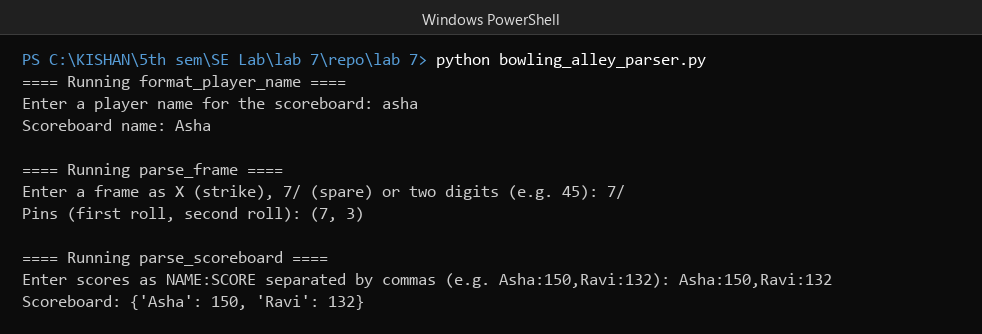
\includegraphics[width=0.9\textwidth]{ss1_buggy_run.png}
  \caption{Running the buggy module with normal input. The happy path works.}
  \label{fig:ss1}
\end{figure}

The problem is that the module only checks nothing. The docstrings say it out loud: ``Assumes name is a non-empty string'', ``Assumes text is a valid frame'', ``Assumes every entry is written as name:score''. Any input outside those assumptions raises an exception.

\section*{Step 3: writing the Hypothesis tests}

I kept the decorator from the starter and filled the three bodies with the try and except shape from the handout, plus one check on the type of the result.

\begin{verbatim}
@given(st.text() | st.none())
def test_format_player_name_no_crash(s):
    # To-Do: Using try and except complete this function.
    try:
        result = format_player_name(s)
    except Exception as e:
        assert False, f"format_player_name crashed with: {e}"
    assert isinstance(result, str)
\end{verbatim}

The other two tests have the same shape. The frame test also checks that the answer is a tuple of length two, and the scoreboard test checks that the answer is a dictionary.

\section*{Step 4: the tests on the buggy module}

Figure~\ref{fig:ss2} shows the run. All three tests fail. Hypothesis prints the smallest input that breaks each one, and it does the shrinking on its own.

The first one is easy to read. Hypothesis started from some random string, kept cutting it down, and ended on \texttt{None}. \texttt{None} has no \texttt{.strip()}, so the function dies with an \texttt{AttributeError}. The same thing happens in \texttt{parse\_frame} and \texttt{parse\_scoreboard}, but those two functions have more than one bug. Hypothesis reported \textbf{5 distinct failures} for \texttt{parse\_frame} and \textbf{3 distinct failures} for \texttt{parse\_scoreboard}. Table~\ref{tab:bugs} lists all the inputs it printed.

\begin{table}[htbp]
  \centering
  \small
  \begin{tabular}{@{}llp{6.4cm}@{}}
    \toprule
    Function & Input found & Error \\
    \midrule
    \texttt{format\_player\_name} & \texttt{None} & \texttt{AttributeError: 'NoneType' object has no attribute 'strip'} \\
    \texttt{parse\_frame} & \texttt{None} & \texttt{AttributeError: 'NoneType' object has no attribute 'strip'} \\
    \texttt{parse\_frame} & \texttt{''} & \texttt{IndexError: string index out of range} \\
    \texttt{parse\_frame} & \texttt{'0'} & \texttt{IndexError: string index out of range} \\
    \texttt{parse\_frame} & \texttt{':'} & \texttt{ValueError: invalid literal for int() with base 10: ':'} \\
    \texttt{parse\_frame} & \texttt{'0:'} & \texttt{ValueError: invalid literal for int() with base 10: ':'} \\
    \texttt{parse\_scoreboard} & \texttt{None} & \texttt{AttributeError: 'NoneType' object has no attribute 'split'} \\
    \texttt{parse\_scoreboard} & \texttt{''} & \texttt{ValueError: not enough values to unpack (expected 2, got 1)} \\
    \texttt{parse\_scoreboard} & \texttt{':'} & \texttt{ValueError: invalid literal for int() with base 10: ''} \\
    \bottomrule
  \end{tabular}
  \caption{Every failing input that Hypothesis shrank to, copied from the run in Figure~\ref{fig:ss2}.}
  \label{tab:bugs}
\end{table}

\begin{figure}[H]
  \centering
  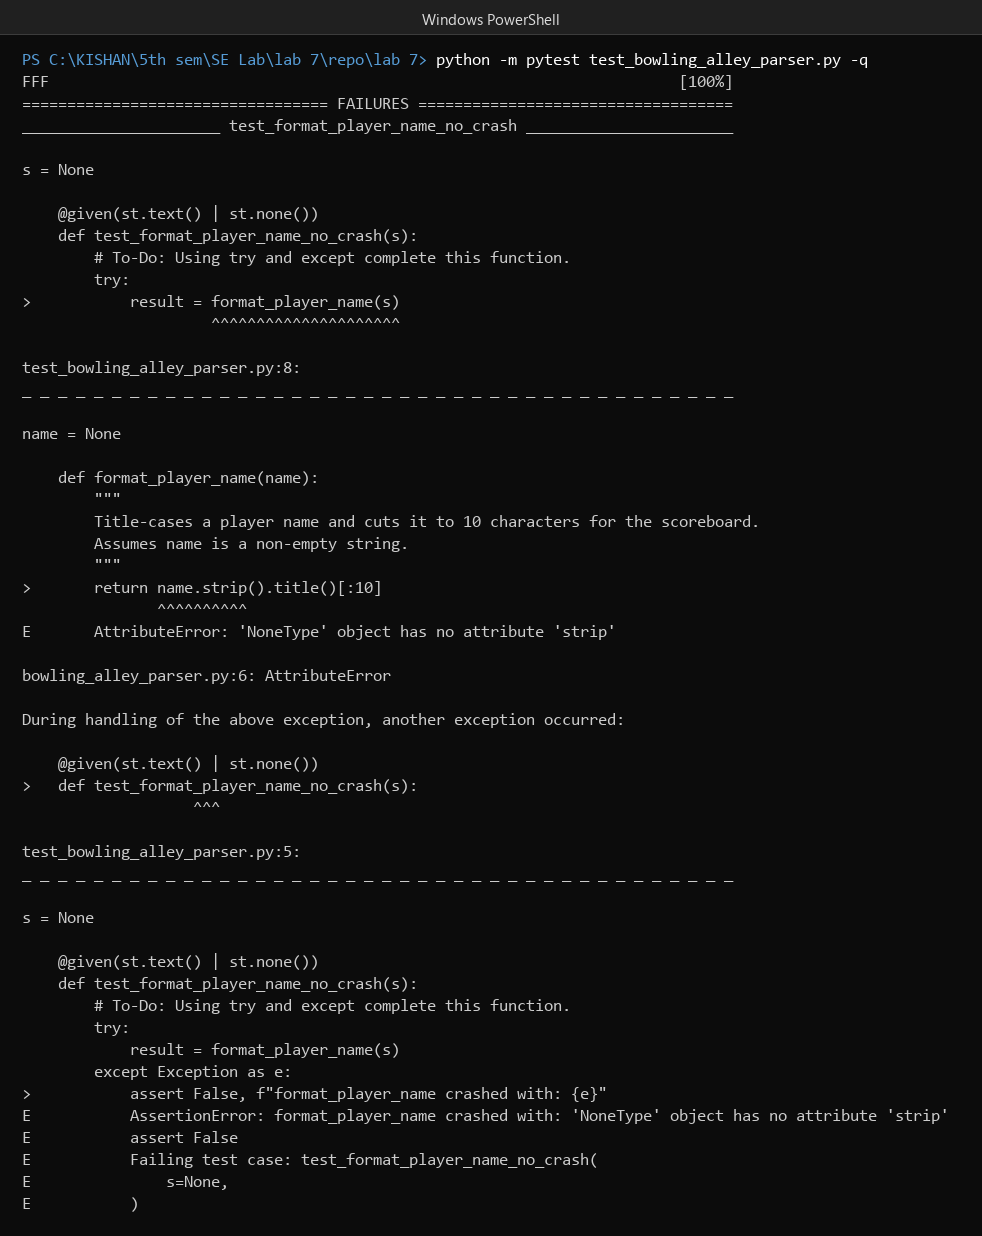
\includegraphics[width=0.8\textwidth]{ss2_tests_failing.png}
  \caption{pytest on the buggy module. Three tests fail, here is the first one with the shrunk input \texttt{s=None}.}
  \label{fig:ss2}
\end{figure}

\section*{Step 5: fixing the module}

I fixed each function the same way. Check the type first, then check the length, then check the characters, and return a safe value instead of raising. For \texttt{parse\_frame} the safe value is \texttt{(0, 0)}, for \texttt{parse\_scoreboard} it is an empty dictionary, and for \texttt{format\_player\_name} it is an empty string. This is the new body of \texttt{parse\_frame}.

\begin{verbatim}
if not isinstance(text, str):
    return 0, 0
text = text.strip().upper()
if text == 'X':
    return 10, 0
if len(text) != 2:
    return 0, 0
digits = '0123456789'
if text[0] not in digits:
    return 0, 0
first = int(text[0])
if text[1] == '/':
    if first == 10:
        return 0, 0
    return first, 10 - first
if text[1] not in digits:
    return 0, 0
second = int(text[1])
if first + second > 10:
    return 0, 0
return first, second
\end{verbatim}

The length check removes the \texttt{IndexError} on \texttt{''} and \texttt{'0'}. The digit check removes the \texttt{ValueError} on \texttt{':'}. I also added two rules that the handout did not ask for but that follow from the game: a spare cannot start with 10 pins, and two rolls in one frame cannot add to more than 10.

\texttt{parse\_scoreboard} skips a bad entry instead of failing the whole line, so one typo does not throw away the other players. \texttt{format\_player\_name} returns an empty string when the name is missing.

\section*{Running the fixed module and re-running the tests}

Figure~\ref{fig:ss3} shows the fixed module on the same kind of input, but with a bad frame and a broken score entry mixed in. Nothing crashes. The name is title cased, the bad frame gives \texttt{(0, 0)}, and the bad score entry is dropped while \texttt{Asha} and \texttt{Ravi} are kept.

\begin{figure}[H]
  \centering
  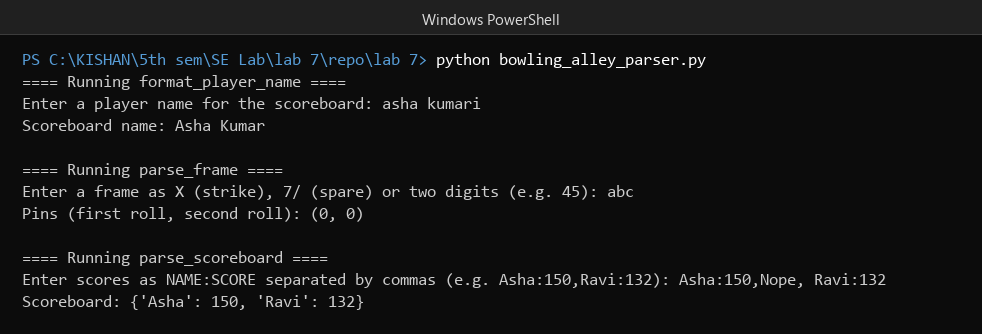
\includegraphics[width=0.9\textwidth]{ss3_fixed_run.png}
  \caption{Running the fixed module with a bad frame and a bad score entry. It does not crash.}
  \label{fig:ss3}
\end{figure}

Figure~\ref{fig:ss4} shows the second test run. All three tests pass.

\begin{figure}[H]
  \centering
  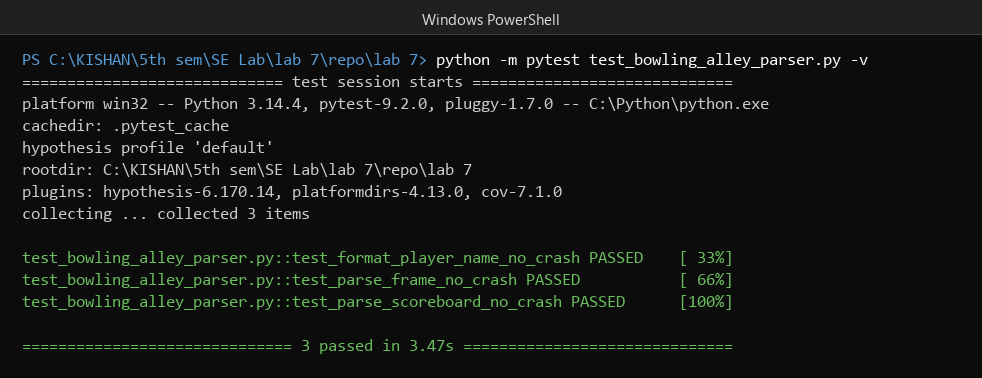
\includegraphics[width=0.9\textwidth]{ss4_tests_passing.png}
  \caption{pytest on the fixed module. Three tests pass.}
  \label{fig:ss4}
\end{figure}

\begin{table}[htbp]
  \centering
  \begin{tabular}{@{}l p{7.2cm} l@{}}
    \toprule
    Run & Command & Result \\
    \midrule
    Buggy module & \texttt{python -m pytest test\_bowling\_alley\_parser.py -q} & 3 failed in 2.78s \\
    Fixed module & \texttt{python -m pytest test\_bowling\_alley\_parser.py -v} & 3 passed in 3.47s \\
    \bottomrule
  \end{tabular}
  \caption{The two test runs, numbers copied from the terminal output.}
  \label{tab:runs}
\end{table}

\section*{Reflection}

\noindent\textbf{1. Which bugs did Hypothesis find that a hand written test would miss?}

When I write tests by hand I think about the mistakes a user makes, like typing \texttt{one,two} instead of numbers. I do not think about \texttt{None} or about an empty string. \texttt{None} is not something a user types into the console, so it looked silly at first. But the same function is what a web form or a file reader will call, and there the missing value is common. The empty string was the best find. \texttt{parse\_frame} reads \texttt{text[0]} and \texttt{text[1]} with no length check, so \texttt{''} and \texttt{'0'} both blow up with an \texttt{IndexError}. I would not have written that test.

\bigskip
\noindent\textbf{2. Why does Hypothesis shrink the failing input, and how did that help?}

The first input that fails is random and can be long, for example a 40 character string with junk in it. That is hard to read and hard to reason about. Hypothesis keeps trying smaller versions while the test still fails, so it ends on the smallest one. For this lab it ended on \texttt{None}, \texttt{''}, \texttt{'0'}, \texttt{':'} and \texttt{'0:'}, which are the small cases I needed. I put them straight into the bug table and then fixed the function for each one. Without shrinking I would have had to cut the string by hand and guess which character matters.

\bigskip
\noindent\textbf{3. What did the fix change, and what can fuzzing still not check?}

Every function now checks the type, the length and the characters before it does any work, and it returns a safe value instead of raising. This makes the module safe to call from any place that passes user input. But fuzzing only checks that the function does not crash. It cannot tell me if \texttt{(0, 0)} is the right answer for a bad frame, because the return type is still a tuple of two numbers. It also cannot check \texttt{main()}, since that needs a real keyboard. The tests check no crash and the return type only, so the actual pin numbers are still on me to verify.

\end{document}
